\section{The sharp central-cut bound}\label{sec:3}

We now apply the certificate framework to a cut through the John center. The proof has a simple overall structure: normalize the old ellipsoid, construct a certificate from its contacts, and bound the determinant of that certificate. A model example will first show where the sharp constant comes from.

\subsection{Statement and normalization}\label{sec:3.1}

\begin{theorem}[{sharp central-cut contraction}]\label{thm-sharp}
Let $K\subset\mathbb R^n$, $n\ge1$, be a convex body, and let $H$ be a closed halfspace whose boundary passes through $c(K)$. Then
\begin{equation}\label{eq:3.1}
w(K\cap H)\le R_nw(K),
\end{equation}
where $R_n$ is given by \eqref{eq:1.3}. For every fixed dimension, there are bodies and central cuts attaining equality.

\end{theorem}

\textbf{Proof arrangement.} The proof is developed in Sections~\ref{sec:3.1}--\ref{sec:3.4} and
completed in Section~\ref{sec:3.4}. It uses Theorem~\ref{thm-frame-bound}, whose proof is deferred to
Section~\ref{sec:8}.

For $n\ge2$, take John coordinates so that $J(K)=B_2^n$, and write
$H=H_v=\{x:v^Tx\le0\}$ with $\|v\|=1$. A candidate $\mathcal E(c,A)$ then has relative volume $\det A$. It is enough to prove $\det A\le R_n$ for every candidate in $K\cap H_v$. The cut body has nonempty interior: it contains, for example, the ball with center $-v/4$ and radius $1/8$.

\subsection{A model that explains the constant}\label{sec:3.2}

We assume $n\ge2$ in the certificate, equality, and stability arguments of Sections~\ref{sec:3.2}--\ref{sec:6}.

Put $b=1/n$ and let $P=I-vv^T$ be the orthogonal projection onto $v^\perp$. Consider the candidate
\begin{equation}\label{eq:3.2}
c_*=-\frac12v,\qquad
A_*=\frac12vv^T+\frac1{\sqrt{1-b}}P,
\qquad \det A_*=R_n.
\end{equation}

Its center moves away from the cutting plane by $1/2$. Its axial semiaxis is $1/2$, so it touches the cut; its transverse semiaxes expand to $(1-b)^{-1/2}$. The product of these lengths is the proposed sharp factor.

Take a regular simplex circumscribed about the unit ball, with unit facet normals $u_1,\ldots,u_{n+1}$. Its standard contact identities are
\begin{equation}\label{eq:3.3}
u_i^Tu_j=-\frac1n\ (i\ne j),\qquad
\sum_i u_i=0,\qquad
\sum_i u_i u_i^T=\frac{n+1}{n}I.
\end{equation}

Thus $\lambda_i=n/(n+1)$ are John weights. Choose $v=-u_1$, so the contact heights are $-1$ and $b$. The three required support values are
\begin{equation}\label{eq:3.4}
\begin{aligned}
(-v)^Tc_*+\|A_*(-v)\|&=\frac12+\frac12=1,\\
u_i^Tc_*+\|A_*u_i\|
&=-\frac b2+\sqrt{\frac{b^2}{4}+\frac{1-b^2}{1-b}}=1
&& (u_i^Tv=b),\\
v^Tc_*+\|A_*v\|&=-\frac12+\frac12=0.
\end{aligned}
\end{equation}

Hence $\mathcal E(c_*,A_*)\subseteq\Delta\cap H_v$ and
$w(\Delta\cap H_v)/w(\Delta)\ge\det A_*=R_n$.

\begin{figure}[tbp]
\centering
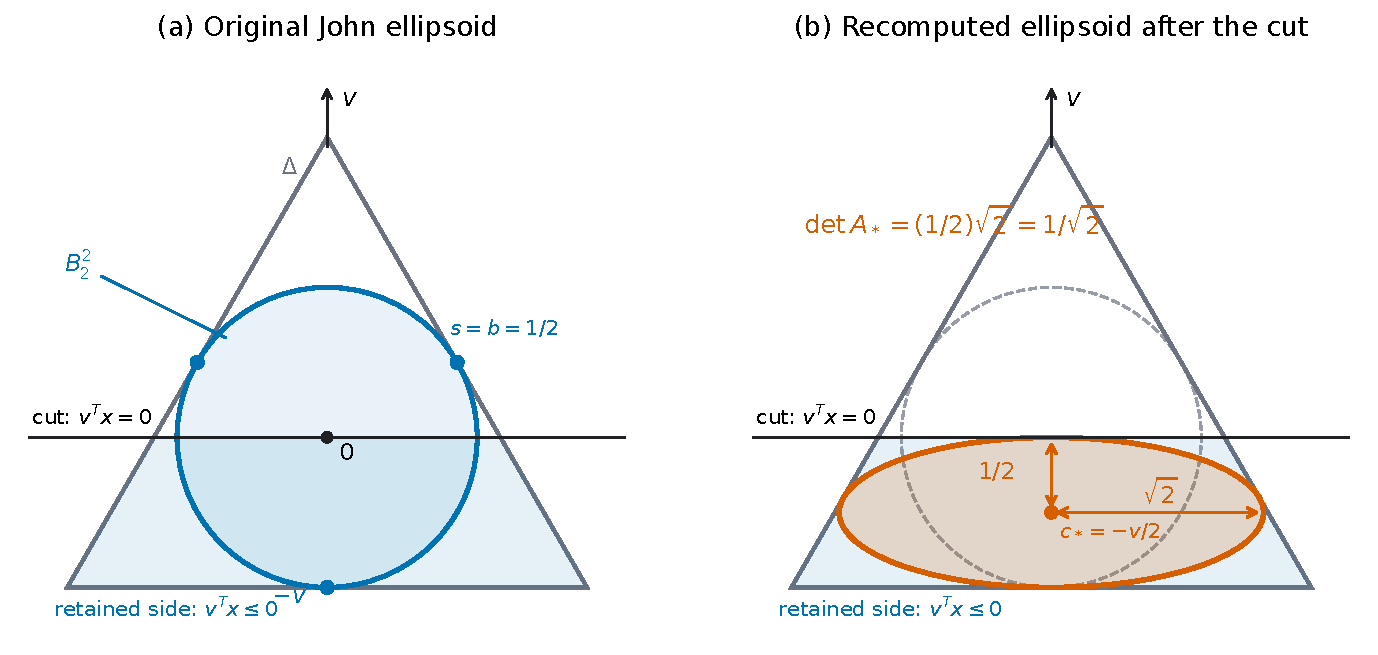
\includegraphics[width=0.98\linewidth]{figures/central_cut.pdf}
\caption{The model in dimension two. The original inball has radius one. The new candidate has semiaxes $1/2$ and $\sqrt2$, so its area ratio is $1/\sqrt2$. The cut bisects the old ellipsoid, but the new ellipsoid can use space in the surrounding body.}\label{fig:1}
\end{figure}

The same support calculation applies to any John frame whose contacts have heights $-1$ and $b$. Section~\ref{sec:5} will describe all such equality configurations. For later use, write the inverse model shape as
$M_0=A_*^{-1}=2vv^T+\sqrt{1-b}\,P$.

\subsection{Constructing a certificate for an arbitrary frame}\label{sec:3.3}

Let $(u_i,\lambda_i)$ be any supporting John frame. Define its axial and transverse components by $s_i=u_i^Tv$ and $y_i=Pu_i$. Old supporting planes carry the index $i$; the added cut has the separate label $0$.

The equality model tells us what the certificate should become:
$M_0=A_*^{-1}$. We seek formulas depending only on the original frame and the
cut, valid for every frame and matching that inverse shape at the model.
The scalar weights enforce balance; the vector directions enforce cone
feasibility and the model support relations.

\textbf{Balance the scalar weights.} Tilting the old weights linearly with the
contact height shifts their weighted normal sum in the direction $-v$.
The new cut, whose normal is $v$, can then restore balance. The John moments
evaluate both sums exactly. Choose
\begin{equation}\label{eq:3.5}
t=\frac{1+b}{2},\qquad
\alpha_i=\lambda_i(1-ts_i)\ge\lambda_i(1-t)\ge\frac{\lambda_i}{4},
\qquad \alpha_0=t.
\end{equation}

The John moments give normalization and balance directly:
\begin{equation}\label{eq:3.6}
\begin{aligned}
\sum_i\alpha_i
&=\sum_i\lambda_i-t\sum_i\lambda_i s_i=n,\\
\sum_i\alpha_i u_i+tv
&=\sum_i\lambda_i u_i-t\left(\sum_i\lambda_i u_iu_i^T\right)v+tv=0.
\end{aligned}
\end{equation}

The cut has right-hand side zero, so its weight does not enter the first sum.
The two identities are exactly the normalization and balance conditions in
\eqref{eq:2.4}. The bound $\alpha_i\ge\lambda_i/4$ keeps every original contact present
and will later control support slacks in the stability argument.
Balance alone allows other values of $t$; matching the equality model fixes
the value in \eqref{eq:3.5}, as explained below.

\textbf{Choose admissible vector directions.} We need unit directions for cone
feasibility: then the provisional choice $q_i=\alpha_i p_i$ lies on the
boundary of the cone. At equality these directions must also be
$A_*u_i/\|A_*u_i\|$, so that the support Cauchy--Schwarz inequality is exact.
The following transformation changes the axial coordinate while preserving
the unit sphere:
\begin{equation}\label{eq:3.7}
a=\frac b{2-b},\qquad k=\sqrt{1-a^2},\qquad
p_i=\frac{(s_i-a)v+ky_i}{1-as_i}.
\end{equation}

Since $\|y_i\|^2=1-s_i^2$ and $1-as_i\ge1-a\ge2/3$, the directions are well defined and
\begin{equation}\label{eq:3.8}
\|p_i\|^2
=\frac{(s_i-a)^2+(1-a^2)(1-s_i^2)}{(1-as_i)^2}=1.
\end{equation}

This is the unit-direction form of a Lorentz transformation. It fixes the
pole $-v$. At the model latitude, the required axial coordinate is
$b/(2+b)$, since $\|A_*u_i\|=1+b/2$ there. Matching
$(b-a)/(1-ab)=b/(2+b)$ gives the chosen $a=b/(2-b)$ and ensures
\begin{equation}\label{eq:3.9}
s_i\in\{-1,b\}\quad\Longrightarrow\quad
p_i=\frac{A_*u_i}{\|A_*u_i\|},
\end{equation}
the contact direction required at the model optimum. The transverse John
moment then shows that matching the transverse part of $M_0$ requires
$1-tb=(1-b)(1+b/2)$, which gives $t=(1+b)/2$.
Thus the parameters in \eqref{eq:3.5} and \eqref{eq:3.7} are fixed by exact model matching,
while the balance and unit-norm identities remain valid for arbitrary frames.

\textbf{The contact defect $\chi$.} To extend model matching to a quantitative
statement for arbitrary contacts, introduce
\begin{equation}\label{eq:3.10}
\chi=\sum_i\lambda_i\frac{(1+s_i)(s_i-b)^2}{1-as_i}.
\end{equation}

The factors $1+s_i$ and $(s_i-b)^2$ make each contribution vanish at the
model pole and latitude. The positive denominator is the same one appearing
in the transformed directions. This choice makes $\chi$ compatible with
the moment calculations of Section~\ref{sec:8}, while preserving
$\chi=0\iff s_i\in\{-1,b\}$ for every contact.

The defect depends only on the original weighted contact geometry and the
cut direction. It will control the determinant excess, identify all equality
frames, and bound weighted distances from those frames. It is therefore the
common geometric quantity behind the sharp bound, equality, and stability.

\textbf{The aggregate matrix $Q$.} Collect the original normals and their
transformed directions into one matrix:
\begin{equation}\label{eq:3.11}
Q=\sum_i\alpha_i u_ip_i^T+t\,vv^T.
\end{equation}

Each term $\alpha_i u_ip_i^T$ records one original constraint and its proposed
dual direction; the term $tvv^T$ represents the new cut.
Thus $Q^T$ is the aggregate of the unrotated vector multipliers.
Like $\chi$, it contains no unknown center or shape of the recomputed ellipsoid.

The following theorem supplies invertibility and a determinant lower bound.
Section~\ref{sec:3.4} will then use one common rotation to turn $Q^T$ into a
positive-definite certificate with the same determinant. This is how the finite
contact construction bounds every feasible cut ellipsoid without solving the
new optimization problem. The central estimate links its volume certificate,
$\log(R_n\det Q)$, to the contact defect $\chi$.

\begin{theorem}[{John-frame certificate bound}]\label{thm-frame-bound}
The matrix $Q$ is invertible with positive determinant. For $d=2-b$,
\begin{equation}\label{eq:3.12}
\frac{\chi}{1500}\le\log(R_n\det Q)\le\frac{\chi}{2d}.
\end{equation}

In particular, $\det Q\ge R_n^{-1}$. Equality in this determinant bound holds if and only if every contact has height $-1$ or $b$; then $Q=M_0$.

\end{theorem}

\textbf{Proof deferred to Section~\ref{sec:8}.} Theorem~\ref{thm-determinant} there is the normalized version
of this estimate. Section~\ref{sec:8.6} proves its equivalence to \eqref{eq:3.12} and completes
Theorem~\ref{thm-frame-bound}, including the equality statement. We first use the result to
finish the geometric proof of Theorem~\ref{thm-sharp}.

\subsection{Completion of Theorem~\ref{thm-sharp}: a common rotation}\label{sec:3.4}

The matrix $Q^T$ need not be symmetric. A single rotation of all the directions produces the positive-definite aggregate required by Lemma~\ref{lem-certificate}. By Theorem~\ref{thm-frame-bound}, the left polar decomposition is well defined:
\begin{equation}\label{eq:3.13}
M=(QQ^T)^{1/2},\qquad U=M^{-1}Q,
\qquad q_i=\alpha_iUp_i,\qquad q_0=tUv.
\end{equation}

Orthogonality follows from
\begin{equation}\label{eq:3.14}
UU^T=M^{-1}QQ^TM^{-1}=I,
\end{equation}
and hence $\|q_i\|=\alpha_i$, $\|q_0\|=t$. The aggregate is
\begin{equation}\label{eq:3.15}
\sum_iq_iu_i^T+q_0v^T=UQ^T=M^{-1}QQ^T=M.
\end{equation}

The scalar weights remain balanced, and
\begin{equation}\label{eq:3.16}
\det M=\sqrt{\det(QQ^T)}=|\det Q|=\det Q\ge R_n^{-1}.
\end{equation}

We now have every part of the certificate: normalization, balance, cone feasibility, positive definiteness, and a lower bound on its determinant.

\begin{proof}[Completion of the proof of Theorem~\ref{thm-sharp}]
Every ellipsoid in $K\cap H_v$ is feasible for the contact polytope and the cut. Lemma~\ref{lem-certificate} gives
\begin{equation}\label{eq:3.17}
\det A\le(\det M)^{-1}\le R_n.
\end{equation}

Since $w(K)=\kappa_n$ in John coordinates,
\begin{equation}\label{eq:3.18}
\frac{w(K\cap H_v)}{w(K)}
=\max_{\mathcal E(c,A)\subseteq K\cap H_v}\det A\le R_n.
\end{equation}

The ratio is affine invariant, proving \eqref{eq:3.1}, and the simplex model attains it. For $n=1$, write $K=[\ell,r]$; then $J(K)=K$, $c(K)=(\ell+r)/2$, and $w(K\cap H)=(r-\ell)/2=w(K)/2$. 
\end{proof}

The proof has also produced a quantitative object: the logarithmic determinant excess in \eqref{eq:3.12}. We next show that this excess is one part of an exact volume deficit. This is the starting point for equality and stability.
